\subsection{Vorüberlegung zur Komplexität}
\label{sec:Komplexity1}
%
\begin{floatingfigure}[hr!]{6cm}
 \centering
         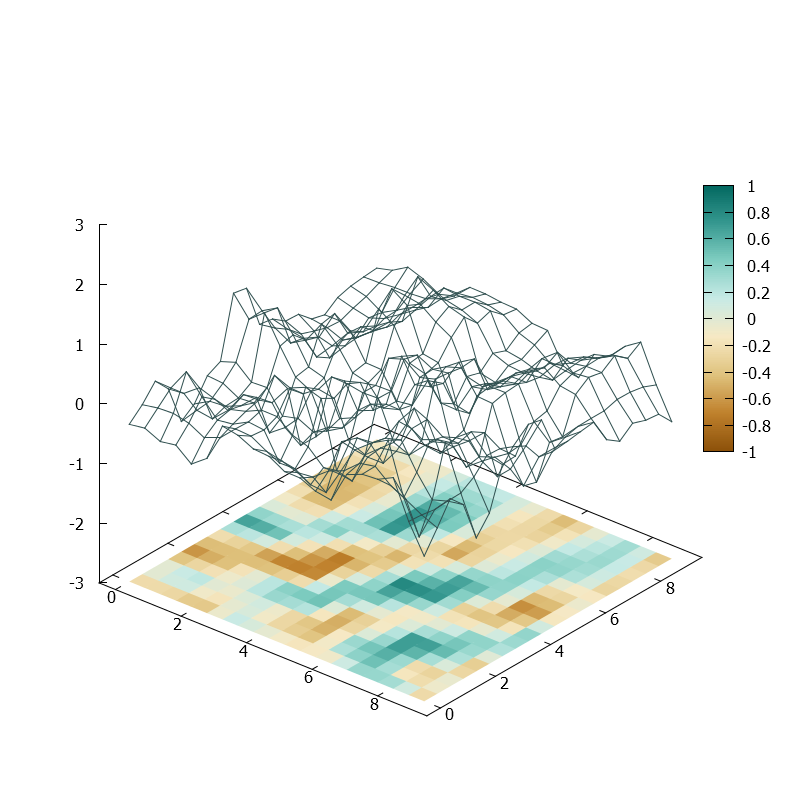
\includegraphics[width=7cm]{img/Plate0_A1.png}
         \caption[Profil einer Phasenmessung]{Normiertes Höhenprofil einer Phasenmessung aus der Sicht von Antenne 1 }
         \label{fig:Plate0_A1_}
\end{floatingfigure}
%
In diesem Abschnitt wird eine Übersicht über die Komplexität des Problems gegeben. In der rechten Abbildung zu sehen ist vergrößert Visualisierung einer typischen Kalibriermessung. Der verwendete Aufbau ist in Abbildung~\ref{fig:Spider1}. gezeigt. Er besteht aus vier Antennen die in einer Ebene angeordnet sind. Es wurde eine reproduzierbare Aufstellung verwendet (Abbildung~\ref{fig:Spider_setup1}) und eine Fläche von $1\times1$ Meter vermessen. Alle $10$ cm wurde eine Messung gespeichert. In der Abbildung kann man deutlich das Verhalten der Phasendaten sehen. Um diesen Verlauf deutlicher zu zeigen wurden die Phasenwerte normiert und als Oberfläche in den Plot gelegt. Am Boden gezeigt ist der Kontur-Plot der Werte. Zwischen den Werten wurde Interpoliert um die Nulldurchgänge deutlicher zu zeigen. Die Übersicht aus der Sicht aller Antennen ist in Abbildung~\ref{fig:Real_Measurements} gezeigt.\\
%

In der Abbildung~\ref{fig:Complexity1} werden die Daten ohne Interpolation dargestellt. Es wurden die Höhenlinien eingezeichnet. Die Anordnung der Plots soll ein Gefühl dafür vermitteln, wie die Messwerte eines Tags sich an unterschiedlichen Postionen und aus sich verschiedener Antennen verhalten.\\
%

Die Darstellung echter Messwerte lässt Rückschlüsse auf die Komplexität des Problems zu. Es ist leicht nachzuvollziehen, dass das Zusammenspiel der Messwerte eine sehr komplexe Szene ergibt. Hier dargestellt ist bereits das Verhalten bei der Verwendung von vier Antennen. Der aktuelle Messaufbau erlaubt sogar acht Antennen. Das ergibt insgesamt eine komplexe Szenerie.\\
%
\begin{figure}[ht!]
        \centering
        \begin{subfigure}[b]{0.4\textwidth}
            \centering
            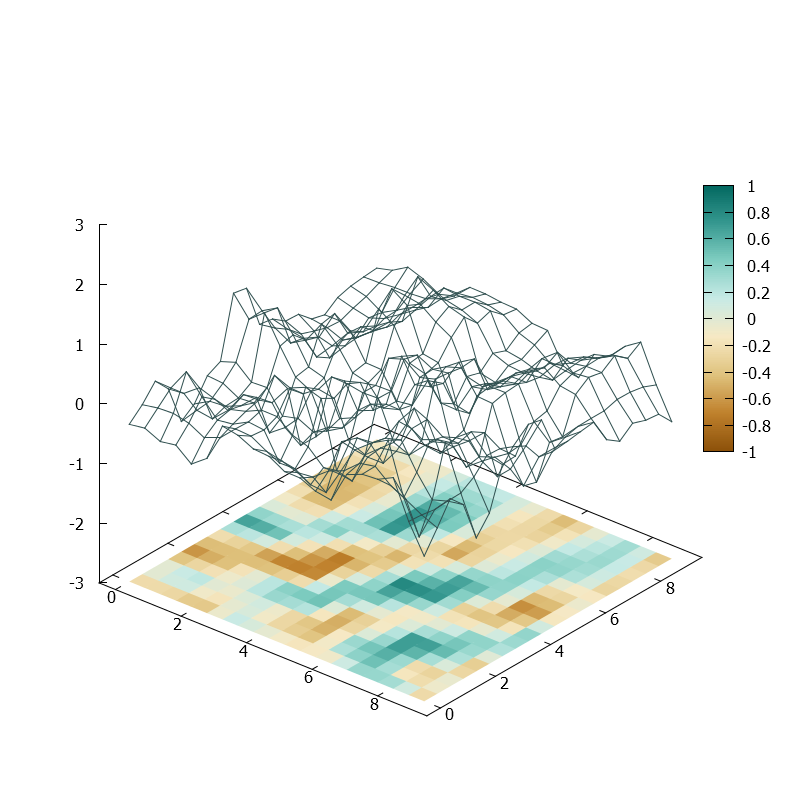
\includegraphics[width=\textwidth]{img/Plate0_A1.png}
            \caption[lorem]{Antenne 1}
            \label{fig:Plate0_A1}
        \end{subfigure}%
\\
        \begin{subfigure}[b]{0.4\textwidth}
            \centering
            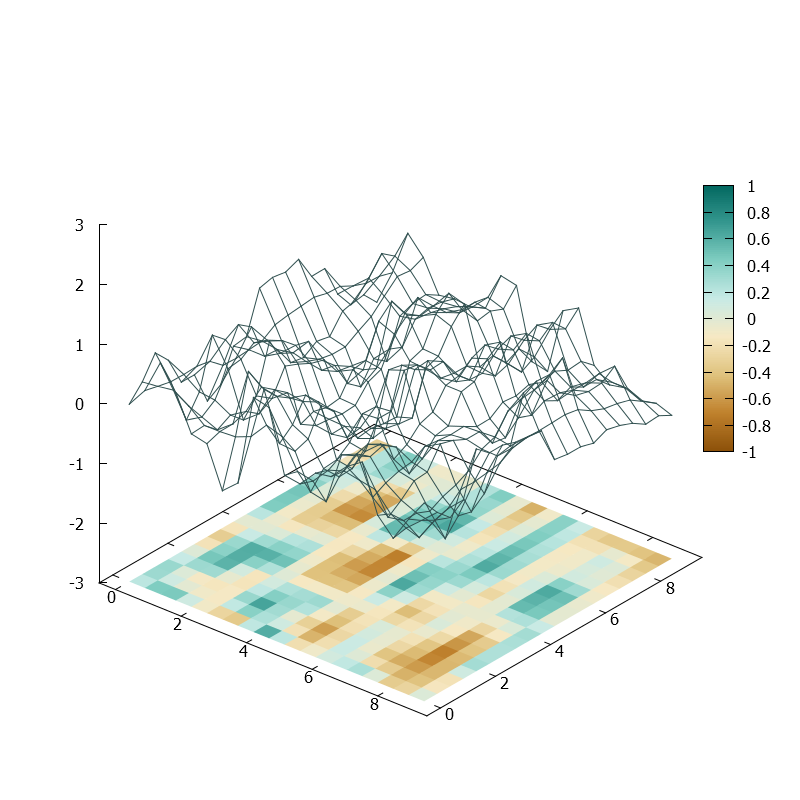
\includegraphics[width=\textwidth]{img/Plate0_A2.png}
          	\caption[Loren ipsum]{Antenne 2}
         	\label{fig:Plate0_A2}
        \end{subfigure}
\qquad\qquad
        \begin{subfigure}[b]{0.4\textwidth}
			\centering
			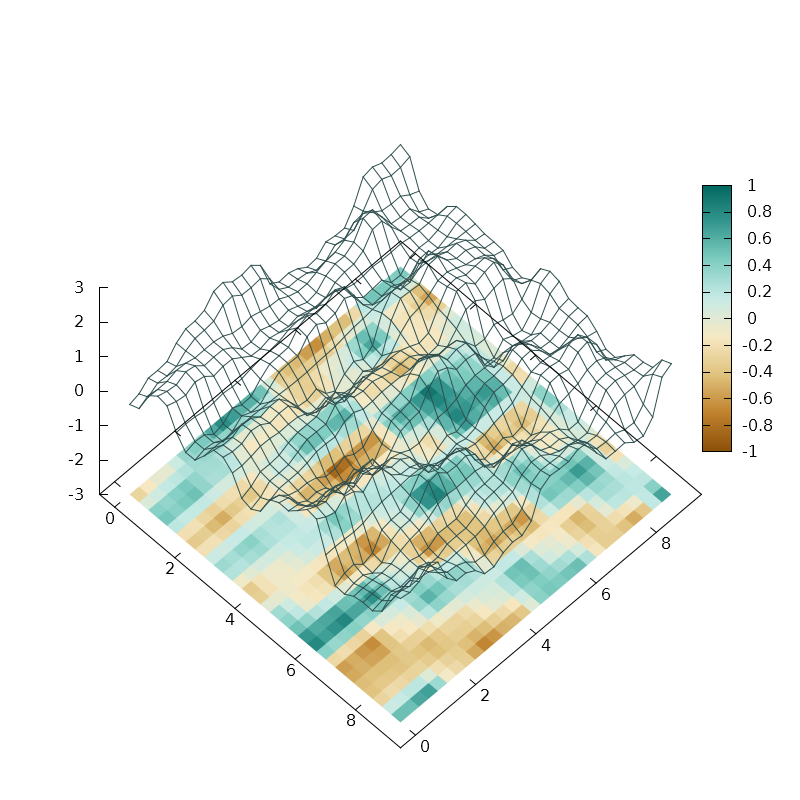
\includegraphics[width=\textwidth]{img/Plate0_A4.png}
			\caption[Loren ipsum]{Antenne 4}
			\label{fig:Plate0_A3}
        \end{subfigure}
\\
        \begin{subfigure}[b]{0.4\textwidth}
			\centering
			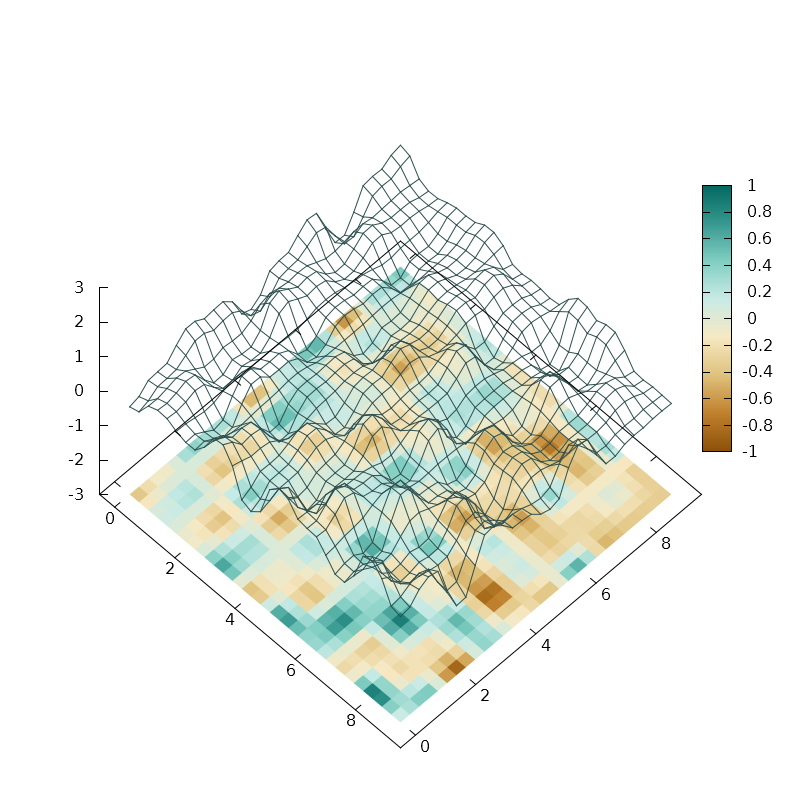
\includegraphics[width=\textwidth]{img/Plate0_A3.png}
			\caption[Loren ipsum]{Antenne 3}
			\label{fig:Plate0_A4}
        \end{subfigure}
        \caption[Reale Messwerte visualisiert]{Blick auf die Messwerte der  Kalibrierplatte aus der "Sicht" der Antennen. Dabei zeigt sich deutlich der Wellencharakter der Messung, dieser ist zu erwarten. Die Messung würden mit bei einer Frequenz von $865,7$ MHz unter Laborbedingungen aufgenommen. }\label{fig:Real_Measurements}
\end{figure}
%
\begin{figure}[ht!]
         \centering
         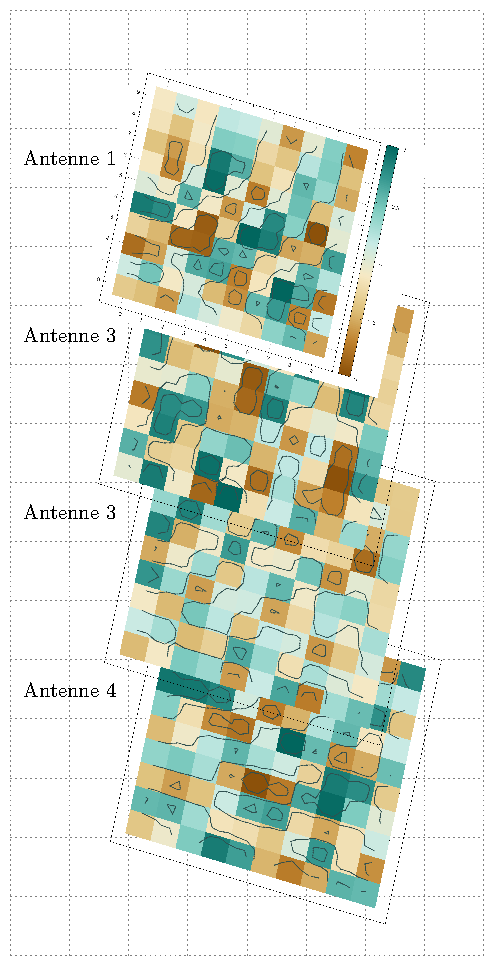
\includegraphics[width=0.6\textwidth]{img/complexitiy1.pdf}
%         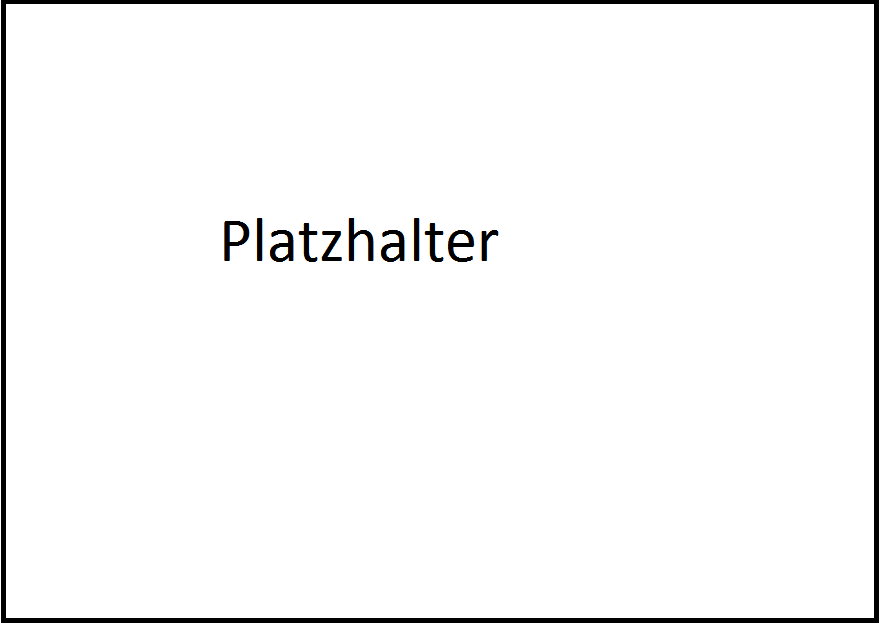
\includegraphics[width=0.7\textwidth]{img/00_placeholder.png}
         \caption[Normierte Messwerte von Kalibriermessung]{Diese Grafik zeigt die Visualisierung von realen Phasen-Messwerten. Die Daten wurden durch Vermessung einer $1\times1$-Kalibrierplatte mit reproduzierbarer Aufstellung\footnote{In dieser Arbeit nicht gezeigt} gewonnen. Die Daten wurden normiert. In jeder Dimension wurden $10\times10$ Werte aufgenommen. Die Darstellung der Phasenwerte erfolgt als Heatmap, es soll qualitativ der Verlauf der Phasenwerte gezeigt werden. Zur Orientierung sind in jedem Plot Höhenlinien eingezeichnet. Pro Plot werden die Daten einer Antenne dargestellt. Die Antenne von der die Daten stammen ist angegeben.}
         \label{fig:Complexity1}
%
\end{figure}


%
\subsection{Entwicklung des Modells}
\label{sec:model_developement}
Im folgenden Abschnitt wird das Modell für die Lösung des Zusammenhangs entwickelt. Zur Veranschaulichung des Sachverhalts dient die Abbildung~\ref{fig:TrilaterationScene}. Dort skizziert ist der Messaufbau mit einem Tag. Die Szene ist in 2D dargestellt die Ableitung des Modells erfolgt direkt für drei Raumkoordinaten.
%
\begin{figure}
	\begin{center}
		\caption[Antennen-Szene mit einem Tag]{2D-Übersicht auf die Szene mit drei Antennen, einem Tag und einer Landmarke. Die Position von $\{A_1,A_3,A_3\}$, sowie der Landmarke, zum Koordinatenursprung sind bekannt. Die Vektoren $r_1,r_2,r_3$ sind die gemessene Entfernung zu einer Antenne. Die Landmarke wird im späteren Verlauf eine Antenne sein, die ihrerseits ein gemessene Entfernung $r_0$ produziert. Der Schnittpunkt aller Kreise ist die Lösung der gemessenen Entfernung und der geom. Anordnung, die sich für die Position des Tags ergibt.} 
		\label{fig:TrilaterationScene}
		\begin{tikzpicture}[
    scale=1,
    axis/.style={thick, ->, >=stealth'},
%    vector/.style={thick, ->,-latex, >=stealth'},
%    antenna/.style={thick},
     important line/.style={thick},
     antenna/.style={thick, cyan!70},
%    dashed line/.style={dashed, thin},
%    pile/.style={thick, ->, >=stealth', shorten <=2pt, shorten
%    >=2pt},
%    every node/.style={color=black},
%    main node/.style={circle,fill=blue!20,draw},
%    help lines/.style={gray,very thin}
    ]
    % axis
    \draw[axis] (-.1,0)  -- (1,0) node(xline)[right] {$x$};
    \draw[axis] (0,-.1) -- (0,1) node(yline)[above] {$y$};

	\draw[gray, very thin, dotted] (0,0) grid (15,6);

	\coordinate (A1_start) at (4,3);
	\coordinate (A1_end) at (4,4);
	\coordinate (A2_start) at (7,5);
	\coordinate (A2_end) at (8,5);
	\coordinate (A3_start) at (8,1);
	\coordinate (A3_end) at (8,2);

	\coordinate (A1_end_) at ($(A1_start)!1!-10:(A1_end)$);
	\coordinate (A2_end_) at ($(A2_start)!1!-10:(A2_end)$);
	\coordinate (A3_end_) at ($(A3_start)!1!-35:(A3_end)$);
	
	\coordinate (Tag_0) at (6,2);
	\coordinate (REF_0) at (12,5);
	\coordinate (Int1) at ($(A1_start)!.5!(A1_end_)$);
	\coordinate (Int2) at ($(A2_start)!.5!(A2_end_)$);
	\coordinate (Int3) at ($(A3_start)!.5!(A3_end_)$);
	
	\begin{scope}
		\node [draw,orange!50,dashed] at (Int1) [circle through={(Tag_0)}] {};
		\node [draw,orange!50,dashed] at (Int2) [circle through={(Tag_0)}] {};
		\node [draw,orange!50,dashed] at (Int3) [circle through={(Tag_0)}] {};
	\end{scope}
	
	\draw[antenna] (A1_start) node[font=\scriptsize,black,below] {$A_1$} -- ($(A1_start)!1!-10:(A1_end)$);
	\draw[antenna] (A2_start) node[font=\scriptsize,black,above] {$A_2$}-- ($(A2_start)!1!-10:(A2_end)$);
	\draw[antenna] (A3_start) node[font=\scriptsize,black,below] {$A_3$}-- ($(A3_start)!1!-35:(A3_end)$);
	
	\node [green!60!black!90, right,font=\scriptsize ] at (REF_0) {$\text{Landmarke}@(x_0,y_0,z_0)$};

	\draw[latex-latex] (Tag_0) -- node[sloped,above,midway] {$r_1$}(Int1);
	\draw[latex-latex] (Tag_0) -- node[sloped,above,midway] {$r_2$}(Int2);
	\draw[latex-latex] (Tag_0) -- node[sloped,above,midway] {$r_2$}(Int3);
	\draw[-latex,dashed,green!60!black!90] (REF_0) -- node[sloped,above,midway] {$r_0$}(Tag_0);
	
	\draw[ -latex,violet!60,font=\scriptsize,dotted] (REF_0) -- node[sloped,above,midway] {$d_{10}$}(Int1);
	\draw[ -latex,violet!60,font=\scriptsize,dotted] (REF_0) -- node[sloped,above,midway] {$d_{20}$}(Int2);
	\draw[ -latex,violet!60,font=\scriptsize,dotted] (REF_0) -- node[sloped,above,midway] {$d_{30}$}(Int3);
		
	\fill[red!70] (Tag_0) circle [radius=2pt];
	\node[font=\scriptsize,black,below] at (Tag_0) {$Tag$} ;
	\fill[green!60!black!90] (REF_0) circle [radius=2pt];
	
\end{tikzpicture}



%		
	\end{center}
\end{figure}
%
Folgende Nomenklatur und Symbole gelten für diesen Abschnitt:
\begin{itemize}[itemsep=0mm]
	\item	$r_{k}$ := Abstand vom Tag zur Antenne
	\item	$d_{kJ}$ := Abstand zur Landmarke
	\item	$N_0:=$ Menge der verfügbaren Antennen $N=\{1,..,8\}$
	\item	$N:=$ Menge der Antennen die für die Optimierung verwendet werden können ($N \subseteq N_0$)
	\item	$N':=$ Menge der Antennen die für die Optimierung verwendet werden ($N' \subseteq N$)
%	; Dabei ist $|N'| \geq 3$
%	\item	Es gilt $|N'| \geq |N| \geq |N_0|$   
	\item	$j$ ist der Index der Referenzantenne, es gilt $j = \{1,2,..,8\}$
	\item	$k$ ist der Index der Antennen einer Messung, es gilt $k = 1,2,..,|N'|-1$
\end{itemize}
%
Wir starten mit der Überlegung über den geometrischen Zusammenhang zwischen der Antennenposition von Antenne $k$ zu der Position des Tags $r_k$:
\begin{align}
	\label{eq:base_vactor}
	r_{k}^2 &= (x-x_k)^2+(y-y_k)^2+(z-z_k)^2
\end{align}
%
Diese Gleichung stellt die Euklidische Vektornorm dar und entspricht der Strecke Antenne-Tag. Für die Ermittelung einer Postion (mit drei Raumkoordinaten) sind drei Antennen Notwendig. Daraus ergibt sich:
%
\begin{itemize}
\item 3 Gleichunge n
\item 3 Unbekannte
\item Quadratisches Gleichungssystem
\end{itemize}
%
Das Gleichungssystem sieht wie folgt aus:
%
\begin{align}
	r_{1}^2 &= (x-x_1)^2+(y-y_1)^2+(z-z_1)^2 \nonumber\\
	r_{2}^2 &= (x-x_2)^2+(y-y_2)^2+(z-z_2)^2 \nonumber\\
	r_{3}^2 &= (x-x_3)^2+(y-y_3)^2+(z-z_3)^2 \nonumber
%	
\end{align}
%
Es ist trivial und wird in verschiedenen Beispielen gezeigt\footnote{z.B. \url{http://en.wikipedia.org/w/index.php?title=Trilateration&oldid=553215995}}, dass man die Koordinaten aus dem quadratischen Gleichungssystem unmittelbar berechnen kann. Es muss jedoch ein quadratisches Gleichungssystem gelöst werden, was zu den bekannten Problematiken führt, insbesondere der Ausschluss mehrdeutiger Ergebnisse. Der Messaufbau der \amedogmbh erlaubt die Verwendung von mehr als 3 Messwertgebern. Diese zusätzliche Informationen lassen sich für eine Linearisierung des Gleichungssystems verwenden. Dieser Ansatz wird für ein Modell im Rahmen dieser Arbeit verwendet und wird im Folgenden beschrieben.\\
%
Von den Antennen sind die Raumkoordinaten ($x,y,z-Koordinaten$) bekannt, bzw. wurden durch Kalibrierung \ref{sec:calibration} in einem vorherigen Schritt bestimmt. Wir können zusätzlich zu notieren:
%
\begin{equation}\label{eq:d_k0}
	d_{kj}^2= (x_k-x_0)^2+(y_k-y_0)^2+(z_k-z_0)^2
\end{equation}
%
Linearisierung des Modells. Dazu wird Gleichung~\ref{eq:base_vactor} in mehreren Schritten umgebaut. Zuerst wird eine neutrale Erweiterung durchgeführt und die Terme geschickt zusammengefasst. Das führt zu:
%
\begin{align}
	r_{k}^2 &= (x-x_k)^2+(y-y_k)^2+(z-z_k)^2 \nonumber \\
	&=(x-x_k+x_0-x_0)^2+(y-y_k+y_0-y_0)^2+(z-z_k+z_0-z_0)^2 \nonumber \\
	&=((x-x_0)-(x_k-x_0))^2+((y-y_0)-(y_k-y_0))^2+((z-z_0)-(z_k-z_0))^2 \nonumber \\ 
	%2 bin. Form
	&=(x-x_0)^2-2(x-x_0)(x_k-x_0)+(x_k-x_0)^2\underbrace{+\dots{}+\dots{}}_\text{y-\& z-Terme analog}
	\label{eq:tri_temp1}
%
\end{align}
%
Um Platz zu sparen sind die y- und z-Terme nicht explizit notiert. Sie ergeben sich durch einfaches Ersetzen der Indizes und werden im Finalen Modell eingefügt. Durch Umstellen von \eqref{eq:tri_temp1} erhalten wir:
\begin{align}
(x-x_0)(x_k-x_0)+\dots{}+\dots{}&=-\frac{1}{2}[r_k^2-(x_k-x_0)^2 -(x-x_0)^2 +\dots{} +\dots{}]\nonumber\\
(x-x_0)(x_k-x_0)+\dots{}+\dots{}&=\phantom{-}\frac{1}{2}[(x_k-x_0)^2 +(x-x_0)^2 +\dots{}+\dots{}-r_k^2]\nonumber
%
\end{align}
%
\begin{multline}\label{eq:rk_final}
(x-x_0)(x_k-x_0)+(y-y_0)(y_k-y_0)+(z-z_0)(z_k-z_0)= \\\frac{1}{2}[(x_k-x_0)^2+(x-x_0)^2-(y_k-y_0)^2+(y-y_0)^2
\\-(z_k-z_0)^2 +(z-z_0)^2-r_k^2]
\end{multline}
%
Vergleich von \eqref{eq:rk_final} mit \eqref{eq:d_k0} bringt: 
%
\begin{multline}
(x-x_0)(x_k-x_0)+(y-y_0)(y_k-y_0)+(z-z_0)(z_k-z_0)= \\\frac{1}{2}[\underbrace{(x_k-x_0)^2+(z_k-z_0)^2+(y_k-y_0)^2}_\text{\boldmath{$d_{kj}^2$}}
\\+\underbrace{(x-x_0)^2+(y-y_0)^2 +(z-z_0)^2}_\text{\boldmath{$r_j^2$}}-r_k^2]
\end{multline}
%
\begin{equation}
(x-x_0)(x_k-x_0)+(y-y_0)(y_k-y_0)+(z-z_0)(z_k-z_0)=\frac{1}{2}[d_{kj}^2+r_{j}^2-r_k^2]\label{eq:rk_final_simplyfied}
\end{equation}
mit 
\begin{equation}\label{eq:c_kj}
\mathbf{c_{kj}}=\frac{1}{2}[d_{kj}^2+r_{j}^2-r_k^2]
\end{equation}
können wir das lineare Gleichungssystem abschließend schreiben:
%
\begin{equation}
%\label{eq:final_trilateration_model}
\mathbf{0}=
\left(
	\begin{array}{ccc}
		x_1-x_j & y_1-y_j & z_1-z_j \\
		x_2-x_j & y_2-y_j & z_2-z_j \\
		x_3-x_j & y_3-y_j & z_3-z_j
	\end{array}
\right)
\left(
   \begin{array}{c}
	   x-x_j\\
	   y-y_j\\
	   z-z_j
   \end{array}
\right)
-
\left(
	\begin{array}{c}
		c_{1j}\\
		c_{2j}\\
		c_{3j}
	\end{array}
\right)
\end{equation}
%
Das Gleichungssystem entspricht ist linear und hat die allg. Form: $\mathbf{0} = \mathbf{Ax}+\mathbf{b}$ es lässt sich mit bekannten Methoden lösen.




{
\small
Folgende Nomenklatur und Symbole gelten für diesen Abschnitt:
%
Wie gezeigt werden konnte\footnote{Wochenbericht KW 20, Anhang B} ergibt sich für den Fall der Trilateration und der Annahme, dass vier Antennen Messwerte liefern, die Gleichung:
\begin{equation}\label{eq:final_trilateration_model}
0=
\left(
	\begin{array}{ccc}
		x_k-x_0 & y_k-y_0 & z_k-z_0 
	\end{array}
\right)
\left(
   \begin{array}{c}
	   x-x_0\\
	   y-y_0\\
	   z-z_0
   \end{array}
\right)
-
\left(
	\begin{array}{c}
		c_{kj}
	\end{array}
\right) 
\end{equation}
%
Dabei ist:
\begin{equation}\label{eq:c_kj}
	c_{kj}=\frac{1}{2}[d_{kj}^2+r_{j}^2-r_k^2]
\end{equation}
%
Ziel dieser Erweiterung ist es, einen Zusammenhang zwischen diesem Modell und der Wellenzahl zu erzeugen. Folgender Ansatz wird gewählt:
	\begin{equation}\label{eq:r_0_varrho} r(\varrho)=\frac{\lambda}{2}\left(\frac{\varrho}{2\pi}+n\right),\\\lambda=\frac{c}{f}, n:= \text{Wellenzahl}
\end{equation}
%
%
Weiterhin ist $\varrho$ die gemessene Phase, die das PRPS-System liefert und $n$ die gesuchte Wellenzahl.\\
Durch einsetzen von \eqref{eq:r_0_varrho} in \eqref{eq:c_kj}, erhalten wir:
\begin{equation}\label{eq:c_k0_extended}
	c_{kj}(\varrho_0, \varrho_k, n_0, n_k) =\frac{1}{2}\left[d_{kj}^2+\frac{\lambda^2}{4}\left(\frac{\varrho_j}{2\pi}+n_0\right)^2-\frac{\lambda^2}{4}\left(\frac{\varrho_k}{2\pi}+n_k\right)^2\right]
\end{equation}
%
Wir stellen Gleichung~\eqref{eq:c_k0_extended} um:
\begin{align}
%	
	c_{kj}(\varrho_0, \varrho_k, n_0, n_k) &= \frac{1}{2}\left\{d_{kj}^2+\frac{\lambda^2}{4}\left[\left(\frac{\varrho_j}{2\pi}\right)^2+2\frac{\varrho_j}{2\pi}n_0+n_0^2 \right.\right.\nonumber\\
	&\phantom{=}\; 
	\left.\left.-\left(\frac{\varrho_k}{2\pi}\right)^2-2\frac{\varrho_k}{2\pi}n_k-n_k^2\right]\right\}\\
%    
    &=\frac{1}{2}\left\{d_{kj}^2+\frac{\lambda^2}{4}\left[\left(\frac{\varrho_j}{2\pi}\right)^2-\left(\frac{\varrho_k}{2\pi}\right)^2 \right.\right.\nonumber\\
    &\phantom{=}\;
   	\left.\left.+2\frac{\varrho_j}{2\pi}n_0-2\frac{\varrho_k}{2\pi}n_k+n_0^2-n_k^2\right]\right\}\\
%	
	&=\frac{1}{2}d_{kj}^2+\frac{\lambda^2}{8}\left[\frac{1}{(2\pi)^2}\left(\varrho_0^2-\varrho_k^2\right) \right.\nonumber\\
	&\phantom{=}\;
	\left. +\frac{1}{\pi}\left(\varrho_0n_0-\varrho_kn_k\right)+\left(n_0^2-n_k^2\right)\right]\label{c_k0_rearragend}
\end{align}
%
Führen wir nun:
\phantomeq{c_{kj}(\varrho_0, \varrho_k, n_0, n_k)}{a_{0k} := \frac{1}{2}d_{kj}^2\nonumber}
\phantomeq{c_{kj}(\varrho_0, \varrho_k, n_0, n_k)}{a_1 := \frac{\lambda^2}{8}\nonumber}
\phantomeq{c_{kj}(\varrho_0, \varrho_k, n_0, n_k)}{a_2 := a_1\frac{1}{\pi}\nonumber}
\phantomeq{c_{kj}(\varrho_0, \varrho_k, n_0, n_k)}{a_{3kj} := a_1\frac{1}{(2\pi)^2}(\varrho_j^2-\varrho_k^2)\nonumber}
%
in Gleichung~\eqref{c_k0_rearragend} ein, erhalten die finale Form der Gleichung:
\begin{equation}
c_{kj}(\varrho_0, \varrho_k, n_0, n_k) = a_{0k}+a_1(n_0^2-n_k^2)+a_2(\varrho_0n_0-\varrho_kn_k)-a_{3kj}\label{c_k0_final_form}   
\end{equation}
%
Die Einführung der Konstanten macht zum Einen die Gleichung übersichtlicher. Zum Anderen können so, mit Blick auf eine spätere Softwareimplementation, Rechenschritte gespart werden. Das sollte sich positiv auf den späteren Berechnungsaufwand auswirken.\\
%
Im Weiteren erkennt man durch scharfes hinsehen das in Gleichung~\eqref{c_k0_final_form}, für $\varrho_k=\text{const.}$ \& $\varrho_0=\text{const.}$ gilt. Das resultiert aus der Tatsache, dass . Es ermöglicht uns zu schreiben:
\begin{equation}
c_{kj}(\varrho_0, \varrho_k, n_0, n_k) = c_{kj}(n_0, n_k)
\end{equation}
%
Im engeren Sinne einer mathematischen Funktion sollten wir die Parameter alle als Argument aufnehmen. Diese Form soll darstellen, welche Größen von Interesse sind. Im späteren Gebrauch wird diese Gleichung in der Optimierung eingesetzt werden.
Für unser Gleichungssystem aus\eqref{eq:final_trilateration_model} ergibt sich:
\begin{equation}\label{eq:wavenumber_trilateration_model}
0=
\left(
	\begin{array}{ccc}
		x_k-x_0 & y_k-y_0 & z_k-z_0 
	\end{array}
\right)
\left(
   \begin{array}{c}
	   x-x_0\\
	   y-y_0\\
	   z-z_0
   \end{array}
\right)
-
\left(
	\begin{array}{c}
		c_{kj}(n_0, n_k)
	\end{array}
\right)
\end{equation}
%
Betrachten wir nun \eqref{eq:wavenumber_trilateration_model}, wählen $N'=4$ (d.h. wir verwenden 4 Antennen) und setzen $j=0$. Wir beschreiben die Konfiguration wie folgt: Antenne 0 ist die Referenz-Antenne und Antenne 0-3 sind Messwertgeber für die Phaseninformation. 
%
\begin{equation}\label{eq:wavenumber_trilateration_model_explicit}
0=
\underbrace{\left(
	\begin{array}{ccc}
		x_1-x_0 & y_1-y_0 & z_1-z_0 \\
		x_2-x_0 & y_2-y_0 & z_2-z_0 \\
		x_3-x_0 & y_3-y_0 & z_3-z_0 
	\end{array}
\right)}_{\textbf{A}}
\underbrace{\left(
   \begin{array}{c}
	   x-x_0\\
	   y-y_0\\
	   z-z_0
   \end{array}
\right)}_{\textbf{x}}
-
\underbrace{\left(
	\begin{array}{c}
		c_{10}(n_0, n_1) \\
		c_{20}(n_0, n_2) \\
		c_{30}(n_0, n_3)
	\end{array}
\right)}_{\textbf{b}}
\end{equation}
%
\begin{equation}
\mathbf{b}=
\left(
	\begin{array}{c}
		a_{01}+a_1( n_0^2-n_1^2)+a_2(\varrho_0n_0-\varrho_1n_1)-a_{310} \\
		a_{02}+a_1(n_0^2-n_2^2)+a_2(\varrho_0n_0-\varrho_2n_2)-a_{320} \\
		a_{03}+a_1(n_0^2-n_3^2)+a_2(\varrho_0n_0-\varrho_3n_3)-a_{330}
	\end{array}
\right)
\end{equation}
%
Das Ergebnis ist ein um $\varrho$ und $n$ erweitertes Gleichungssystem. Zusätzlich enthält  es mehrere geometrische Konstanten ($a_{0k}, k=\{1,..,N-1\}$), mehrere Phasen-Konstanten ($a_{3k0}, k=\{1,..,N-1\}$), sowie zwei allgemeine ($a_1$ und $a_2$). Allgemeiner formuliert ergibt sich:
%
\begin{multline}\label{eq:final_equation}
0=
\left(
	\begin{array}{ccc}
		x_k-x_0 & y_k-y_0 & z_k-z_0 
	\end{array}
\right)
\left(
   \begin{array}{c}
	   x-x_0\\
	   y-y_0\\
	   z-z_0
   \end{array}
\right) \\
-
\left(
	\begin{array}{c}
		a_{0k}+a_1(n_0^2-n_k^2)+a_2(\varrho_0k_0-\varrho_kn_k)-a_{3kj}
	\end{array}
	\right)
\end{multline}
%
Aus Gleichung~\eqref{eq:final_equation} ist durch eine geeignete Wahl von $N'=\{4,..,N\}$ sofort ersichtlich wie viele Veränderliche sich für eine gewählte Konstellation an Antennen ergeben. Für $k$ gilt in diesem Fall $k=\{1,..,N'-1\}$.\\
%
Beispielsweise ergibt sich für das Modell aus Gleichung~\eqref{eq:final_equation} mit $N'=4$, insgesamt 7 Variablen ($\mathbf{x},n_0,n_1,n_2,n_3$) . Analog würde sich für ein Modell mit allen 8 Antennen, 11 Variablen ($\mathbf{x},n_0,..,n_7$) ergeben.
}
{
Abschließend soll das das bisher verwendete Modell umgeschrieben werden, damit die Allgemeingültigkeit darin enthalten ist.
\begin{align}
%
%\mathbf{0}&=\mathbf{A}\mathbf{x}-\mathbf{b}\\
%
\mathbf{A}&=
\left(
	\begin{array}{cccccc}
		x_k-x_0 & y_k-y_0 & z_k-z_0 & \sum_{i=1,j=0}^{k}(-a_1\delta_{ij}) &  -a_2\Theta_0 & \sum_{i=1,j=0}^{k}(a_2\Theta_k\delta_{ij})
	\end{array}
\right)\nonumber\\
%
\mathbf{x}&=
\left(
   \begin{array}{c}
	   x-x_0\\
	   y-y_0\\
	   z-z_0\\
	   n_0^2-n_k^2\\
	   n_0\\
	   n_k
   \end{array}
\right)\nonumber\\
%
\mathbf{b}&=
	\begin{array}{c}
		a_{0k}-a_{3kj} 
	\end{array}
	= c_{kj}'\nonumber
\end{align}
%
Dabei steht $\delta_{ij}$ für den bekannten Kronecker-Operator und bedeutet:
\begin{equation*}
\delta_{ij} = \begin{cases}1 ~\text{für}~ i=j\\ 0 ~\text{für}~ i\neq j\end{cases}
\end{equation*}
%
Im Expliziten sehen die Matrix $\mathbf{A}$ und der Vektor $\mathbf{b}$, für denn Fall $N'=3$ und $k=\{1,2,3\}$, wie folgt aus:
%
\begin{multline}
\mathbf{A}=\\
\left(
	\begin{array}{cccccccccc}
		x_1-x_0 & y_1-y_0 & z_1-z_0 & -a_1 & 0 & 0 & -a_2\Theta_0 & a_2\Theta_3 & 0 & 0 \\
		x_2-x_0 & y_2-y_0 & z_2-z_0 & 0 & -a_1 & 0 & -a_2\Theta_0& 0 & a_2\Theta_3 & 0 \\
		x_3-x_0 & y_3-y_0 & z_3-z_0 & 0 & 0 & -a_1 & -a_2\Theta_0& 0 & 0 & a_2\Theta_3
	\end{array}
\right) \nonumber
\end{multline}
%
\begin{equation}
\mathbf{x}=
\left(
	\begin{array}{c}
		x-x_0	\\
		y-y_0	\\
		z-z_0	\\
		n_0^2-n_1^2	\\
		(\dots)	\\
		n_0^2-n_3^2	\\
		n_0 \\
		n_1	\\
		(\dots)	\\
		n_3	
	\end{array}
\right)\nonumber
\end{equation}
%
\subsubsection{Bemerkungen - Finales Modell}
%
Das Ergebnis ist eine $3\times10$ Matrix und ein $1\times10$ Vaktor. Es ist möglich diesem Modell eine beliebige Anzahl an Antennen hinzuzufügen. Fügt man eine Antenne zur Berechnung hinzufügen würde sich die Matrix $\mathbf{A}$ um zwei Spalten und eine Zeile erweitern, der Vektor $\mathbf{x}$ analog um 2 Zeilen.

}
%
\subsection{Erweiterte Betrachtung der Kondition}
Die vorgestellte erweiterte Form des Modells erleichtert Implementation und Verifikation. Große Teile des Modells sind statisch (vgl. \ref{eq:block_matrix_form}) und können im Voraus berechnet werden. Es sind nun auch die gemessenen Phasenwerte Teil des Modells, genauer: der Matrix $\mathbf{A}$. Im Folgenden werden die Auswirkungen auf die Kondition der Matrix betrachtet. Dazu wird Untersucht inwieweit die Zerlegung in Blockmatrizen und die Untersuchung der Kondition dieser eine Abschätzung der vollständigen Konditionszahl im Allgemeinen darstellt. 
%
\begin{equation}
\label{eq:block_matrix_form}
\mathbf{A}=\bigg( \mathbf{Z}\quad \mathbf{P}\quad \mathbf{V}\bigg)
\end{equation}
%
Dabei ist:
\begin{equation}
\mathbf{Z} \in \mathbb{R}^{3x3} \quad \mathbf{P} \in \mathbb{R}^{3x3} \quad \mathbf{V}\in \mathbb{R}^{4x3}
\end{equation}
%
Die Matrizen $\mathbf{Z}$ und $\mathbf{P}$ sind statisch. Hingegen enthält die Matrix $\mathbf{V}$ die gemessenen Phasenwerte $\Theta_k$ der Antennen für diese Konfiguration. \\
%
Die Abbildung~\ref{fig:CondNumberAnalyze} zeigt die bereits angestellte Untersuchung zu dieser Überlegung. Abbildung~\ref{fig:AnalyzeOf3x3} stellt die Konditionszahl der rein geometrischen $3\times3$-Matrix dar. In der Abbildung~\ref{fig:AnalyzeOf10x3} sehen wir die Kondition der erweiterten Matrix. Neben der geometrischen sind auch die beiden anderen Blockmatrizen in diese Konditionsbetrachtung eingeflossen. Als zusätzliche Angabe wird ist sind die Skalierungsfaktoren angegeben. Legt man beide Grafiken übereinander erkennt man:
\begin{enumerate}
\item Geometrisch gut konditionierte Konfigurationen (linke Grafik), bleiben im erweiterten Modell (rechte Grafik) weiterhin gut konditioniert.
\item Die Konditionszahl der \textit{schlechteste} ist wesentlich kleiner (ca. Faktor $10$) als im rein geometrischen Modell
\end{enumerate}
%
\begin{figure}[h]
         \centering
	     \caption{Analyse der Konditionszahlen aller möglichen Matrizen für den Messaufbau; Die Konditionszahl ist für jede mögliche Permutation an Messantennen für eine Referenzantenne angegeben}\label{fig:CondNumberAnalyze}
         \begin{subfigure}[h]{0.5\textwidth}
                 \centering
                 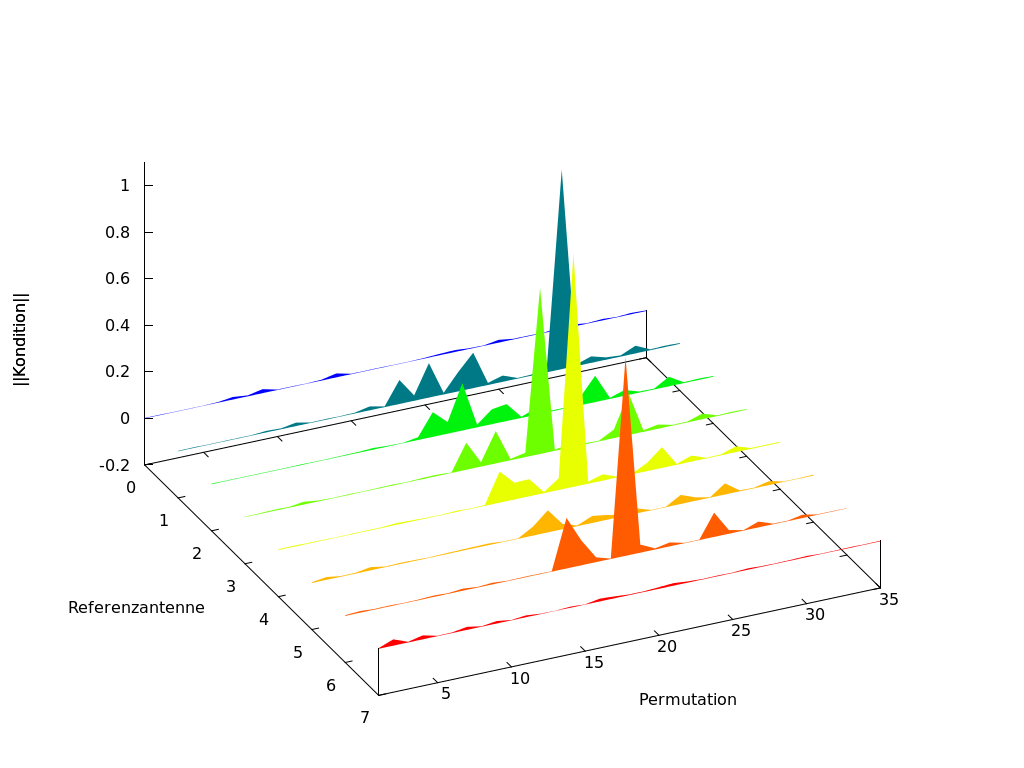
\includegraphics[width=\textwidth]{img/fenceModell3x3.png}
                 \caption{Konditionszahl der rein geometrischen $3\times3$ Matrix normiert auf den größten vorkommenden Wert ($=2149,16                 $)}
                 \label{fig:AnalyzeOf3x3}
         \end{subfigure}
%         
         \begin{subfigure}[h]{0.5\textwidth}
                 \centering
                 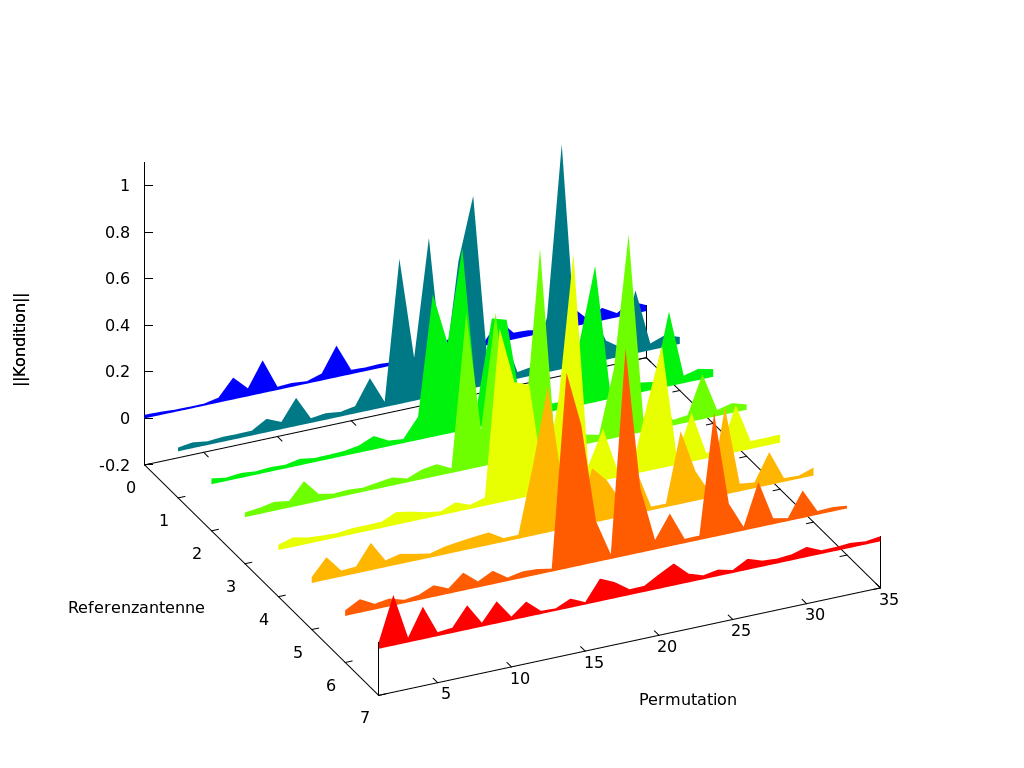
\includegraphics[width=\textwidth]{img/fenceModell9x3.png}
                 \caption{Konditionszahl der $10\times3$ Matrix normiert auf den größten vorkommenden Wert ($=257,13$); In dieser Konfiguration sind die Konstanten ($a_1$ \& $a_2$) sowie die variablen, gemessenen Phasen $\Theta_k$ enthalten}
                 \label{fig:AnalyzeOf10x3}
         \end{subfigure}
%
\end{figure}
%
Aus der Grafik lässt sich entnehmen, dass es für jede Referenzantenne aus der Geometrie alleine gute Konfigurationen existieren. Aus diesen Erkenntnissen kann in späteren Aufbauten, die Position der Antennen optimiert werden. Diese Verfahren wird in Abschnitt~\ref{sec:Calibration_Optimaztion} weiter beschrieben.
%
%- Section 2.3 --------------------------------------------------------------
\subsection{Weitere Anwendung der Konditionszahl}
Weitere Anwendungen, die sich aus der Konditionszahl der Matrix ableiten, sind denkbar. Für die FPGA-Software ist, parallel zu diesem Projekt, eine intelligente Umschaltung der Antennen in der Planung. Die Kondition der geometrische Matrix verändert sich nach dem Kalibrieren nicht mehr. Dadurch und durch die oben beschriebenen Überlegungen kann statisch eine Abschätzung für die Konditionszahl, von zwei der drei Blockmatrizen, im Vorfeld erstellt werden. Die Konditionszahl dient zum Steuern der Umschaltung. Ordner man die möglichen Konfiguration anhand ihrer Konditionszahl (niedrigste zuerst) in einer statischen Liste an so kann im FPGA eine einfache, schlaue Umschaltung implementiert werden. Diese würde immer dafür sorgen, dass Messdaten von einer Konfiguration bevorzugt werden, die eine niedrige Konditionszahl hat und somit relativ sicher zu einer guten Lösung führen. Diese überlegungen werden im Rahmen dieser Arbeit nicht näher beschrieben.\\
Eine Weitere Anwendung ergibt sich für die Kalibrierung. Der Aufbau der Antennen kann unter Berücksichtigung der Kondition optimieren. Ziel der Optimierung wäre es durch eine geeignete Positionierung der Antennen, die Anzahl der Antennenpermutationen mit kleiner Konditionszahl zu maximieren.
%
%\subsection{Konkurierende Modelle}
% SuWi - Zeug 
%\lipsum[1-1]
%
\subsection{Betrachtung der Komplexität}
\label{sec:Komplexity2}
%
Im Folgenden wird eine Betrachtung der Komplexität des in Abschnitt~\ref{sec:model_developement} entwickelten Modells präsentiert. Diese Betrachtung ist wichtig für die Parametrisierung des Optimierungsverfahrens sowie für eine Beurteilung der Generellen Lösbarkeit mit den verwendeten Verfahren. Es wird eine Visualisierung des Fitness-Raums vorgestellt und im Vergleich mit sog. Benchmark-Funktionen diskutiert.\\
%

Für die Erstellung der Fitness-Ebenen wurde ein Programmteil (der \textit{FitnessPlaneCalculator}) entwickelt, der ein Modell mit vorgegebenen Daten füttert und den Rückgabewert in eine Datei schreibt. Das Programm lässt sich per Eingabedatei steuern und erlaubt die Definition der Ebenen die dargestellt werden sollen. Es lassen sich immer zwei Variablen der Objektfunktion variieren und der Rest wird dabei auf feste Werte gesetzt. Das erlaubt eine Visualisierung durch eine 2D-Heatmap (siehe folgende Plots). Aus der Visualisierung können Rückschlüsse auf die Gestalt der Fitnessebene gezogen werden.\\
%

Die Parameter wurde für diese Plots so gewählt das sie über einen Bereich iterieren, indem die richtige Lösung liegen sollten. Da nur drei Parameter variiert werden, werden die übrigen vier auf analytisch bestimmte, wahre Werte gesetzt. Diese sind in Tabelle~\ref{tab:complexity1} zusammen mit den wahren Werten aufgeführt.\\

%
\begin{figure}[h!]
  \caption[Fitness Ebenen Heatmap]{Diese Grafik zeigt die Fitnessebenen des Problems für eine Anordnung aus vier Antennen und einem Sweep über die $x-y$ - Ebene. Jeder Plot ist für einen festen Wert $z$ erstellt worden. In der Oberen linken Ecke beginnend und nach rechts laufend. Die $x, y$-Werte wurden über ein Intervall von $[-5,5]$ m und mit einem Inkrement von $0.2$ variiert. Daraus ergibt eine für die Abschätzung der Gestalt der Fitnessebene ausreichende Datengrundlage. Die $z$-Werte der $16$-Plots stammen aus dem Intervall $[-7,-7]$ mit einem Inkrement von $1$. Bereits in dieser Ansicht, ist zu erkennen, dass der Verlauf sehr Flach ist. Eine Schlucht bildet sich etwa in Nord-Süd-Richtung aus. Jeweils verzeichnet ist das lokale Minima ($+$) eins Plots, sowie die Höhenlinien\footnote{Die Höhenlinien sind für diskrete Werte ${0,1,10,40,50,100,200,500,1000}$ erstellt worden}. Die farbliche Kodierung gibt den Fitnesswert an diesem Punkt an. Die Fitnesswerte wurden normiert und um den Wert ihres Minimums verschoben.}
  \begin{center}
    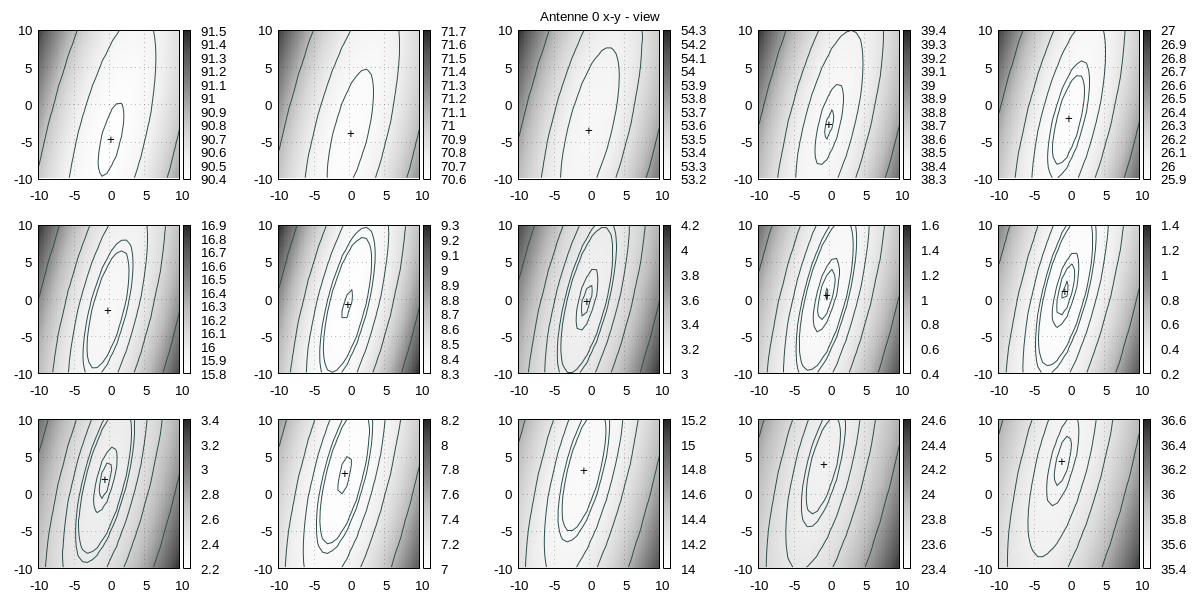
\includegraphics[width=\textwidth]{img/fitness/xy_a0.png}
  \end{center}
  \label{fig:fitnessplane1-x-y-1}
%
\end{figure}

\begin{figure}[ht!]
  \caption[Fitness Ebenen Heatmap, vergrößert]{Vergrößerung der Fitnessebenen der Antenne 1. Es ist hier deutlich zu erkennen, wie gering die Funktionen ansteigen. Das ist ein Problem für die meisten Algorithmen. Es bleibt zu klären wie sensitiv der Algorithmus auf diesen Umstand reagiert. Es wurde um das lokale Minima zentriert und der Bereich auf}
  \begin{center}
   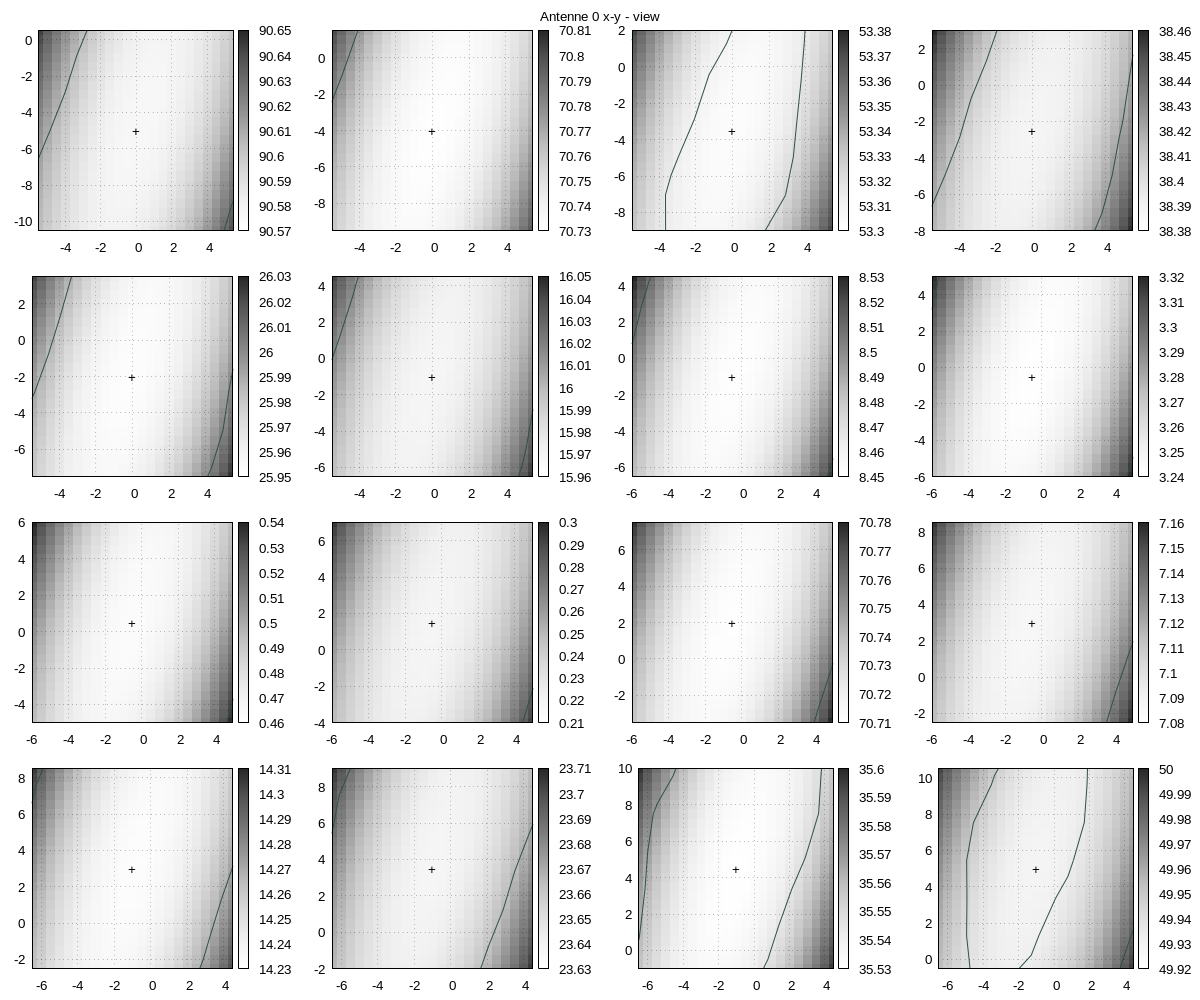
\includegraphics[width=\textwidth]{img/fitness/xy_a0zoomed.png}
  \end{center}
  \label{fig:fitnessplane1-x-y-zoom-1}
%
\end{figure}
%
In den Abbildungen~\ref{fig:fitnessplane1-x-y-1} und \ref{fig:fitnessplane1-x-y-zoom-1} zeigen sich möglicherweise die ersten Probleme für den Algorithmus. Eine große, sehr flache Fitnessebene für verschiedene Parameter ist nicht leicht zu handhaben. Aus dieser Untersuchung geht bereits hervor, dass die Anzahl an Nachkommen groß sein muss. Auch darf die Schrittweite $\sigma$ nicht zu klein werden, damit die Lösung nicht auf der flachen Ebene liegen bleibt. Ein Ähliches Verhalten zeigt sich bei den anderen Antennen und anderen Ebenen. Aufgrund der Komplexität des in dieser Arbeit erstellten Modells \ref{fig:Complexity1} ist bereits dieser Fall recht hochdimensional. Er erreicht $7$ Dimensionen und er kann im Rahmen dieser Arbeit nicht vollständig Untersucht werden. Die Fitness-Plots aller Antennen und für drei Ebenen sind in Anhang~\ref{app:fitness:plots1} zu finden. Eine vollständige Untersuchung ist indes auch nicht notwendig, da der Algorithmus den Suchraum in gewisser Weise untersucht. 
%
\begin{figure}[!h]
	 \caption[Übrige Ebenen für Antenne 1]{Auf diesen Abbildungen zeigen sich die Fitness-Ebenen für die übrigen Ansichten, x-z und y-z. In der oberen Reihe sind Ebenen über den gesamten Bereich, in der Unteren vergrößert dargestellt. Zu erkennen ist ein zum Verlauf der x-y-Ebene sehr ähnliches Bild. Ein flaches, längliches Tal mit Minimum.  }
	 \label{fig:fitnessplanesA1}
     \centering
     \begin{subfigure}[t]{0.4\textwidth}
             \centering
             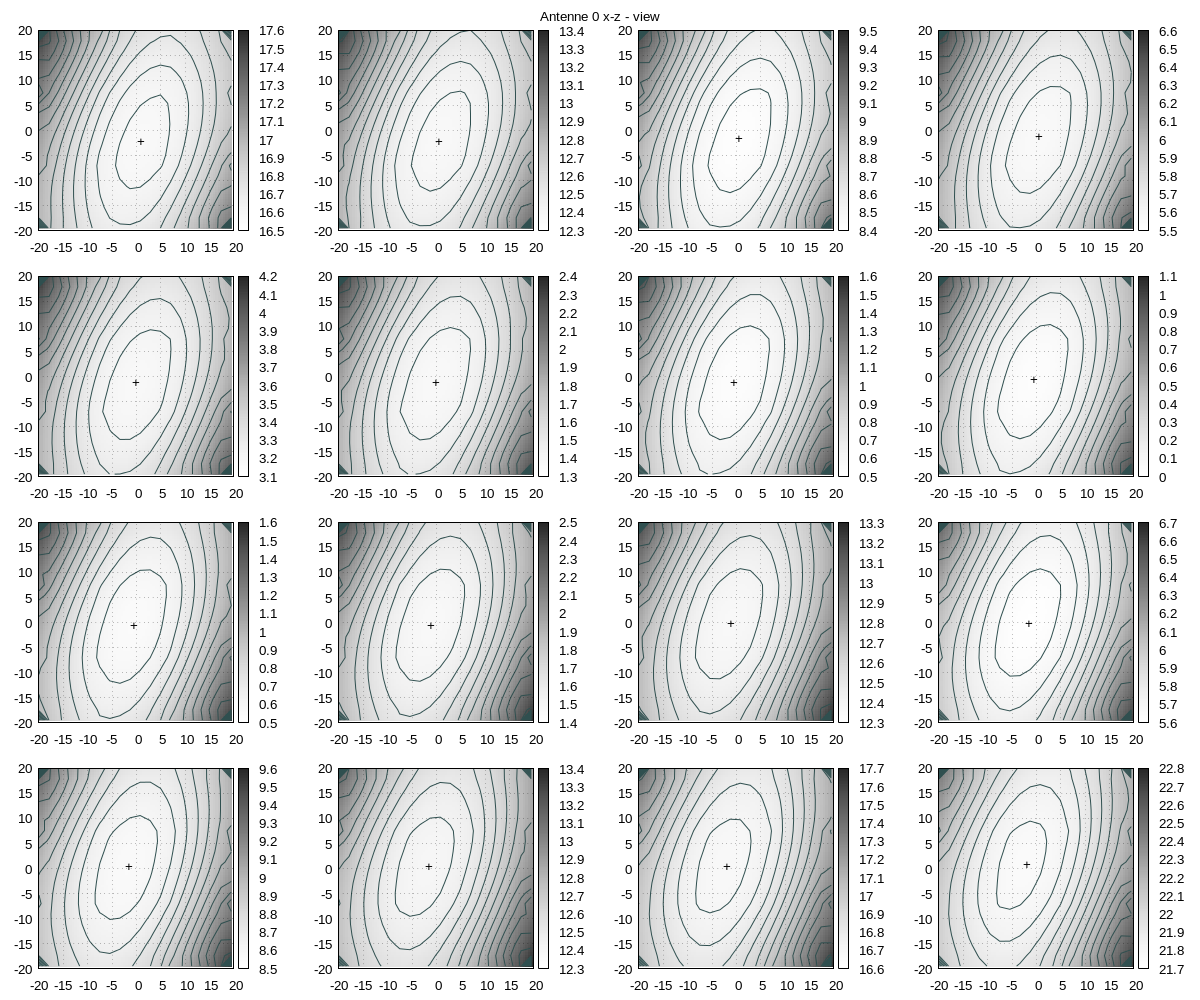
\includegraphics[width=\textwidth]{img/fitness/xz_a0.png}
%             \caption{Statistisch verteilte Endwerte für die Koordinaten der Kalibrierung.}
%             \label{fig:abortedFinal_Calibration_Ant0_ES-boxes}
     \end{subfigure}
     \qquad
     \begin{subfigure}[t]{0.4\textwidth}
			\centering
			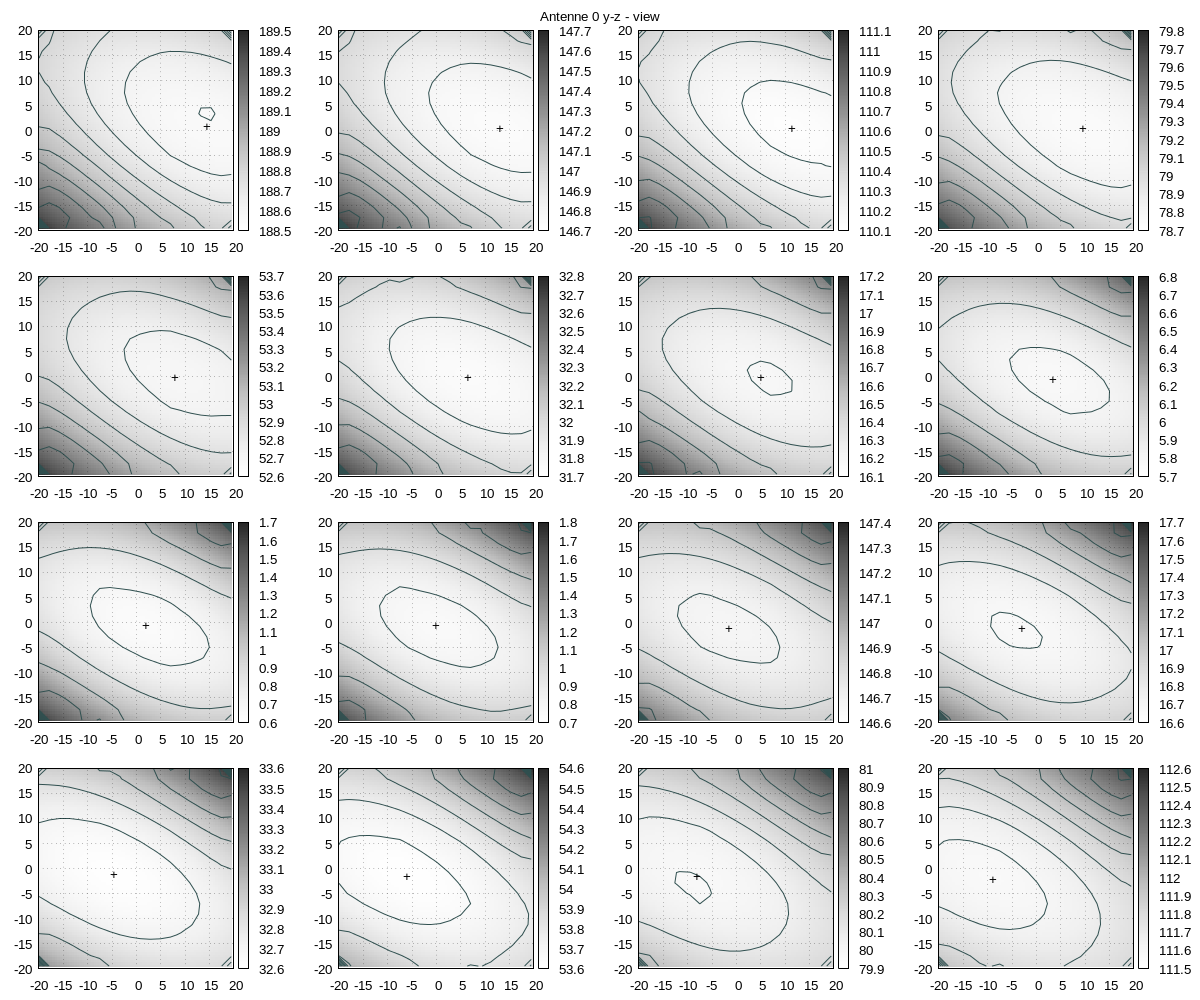
\includegraphics[width=\textwidth]{img/fitness/yz_a0.png}
%			\caption{x-z-Ebene, vergrößert}
%			\label{fig:abortedFinal_Calibration_Ant0_ES-boxes}
	 \end{subfigure}
\\
\vspace{5mm}
     \begin{subfigure}[t]{0.4\textwidth}
			\centering
			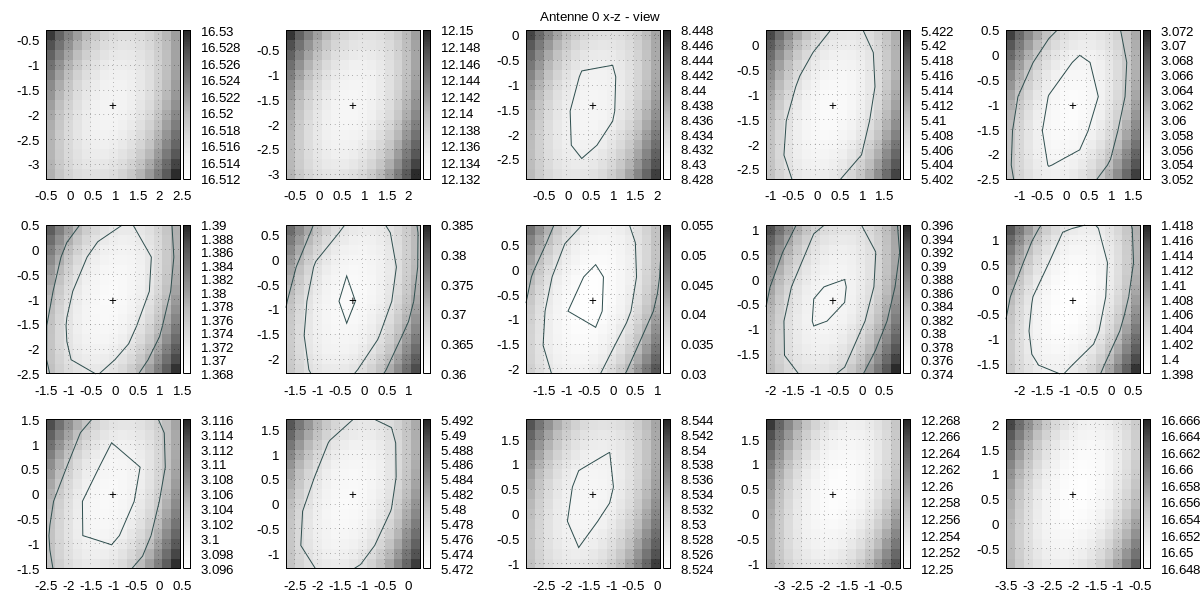
\includegraphics[width=\textwidth]{img/fitness/xz_a0zoomed.png}
%			\caption{x-z-Ebene, vergrößert}
%			\label{fig:abortedFinal_Calibration_Ant0_ES-boxes}
	 \end{subfigure}
	 \qquad
     \begin{subfigure}[t]{0.4\textwidth}
			\centering
			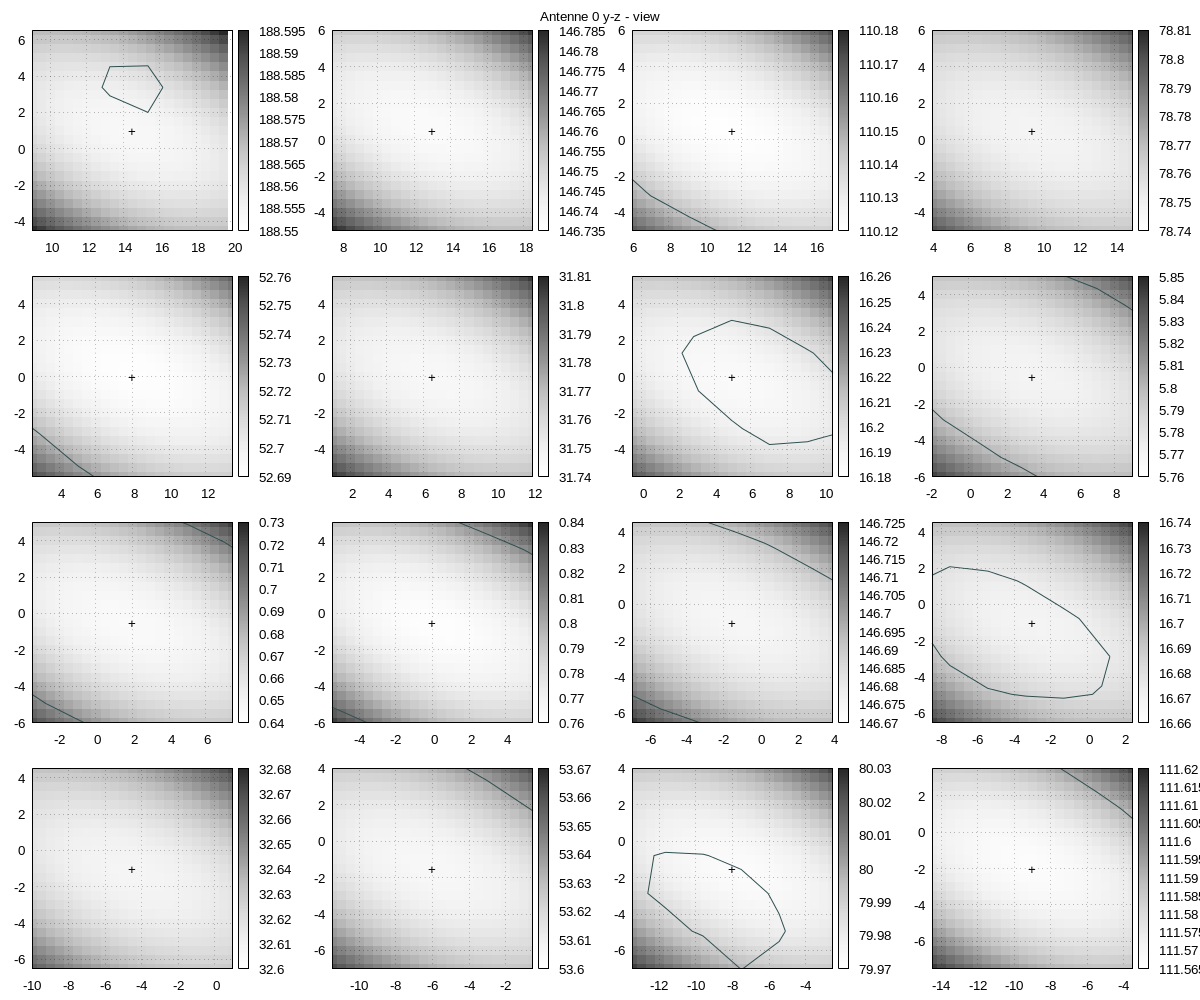
\includegraphics[width=\textwidth]{img/fitness/yz_a0zoomed.png}
%			\caption{x-z-Ebene, vergrößert}
%			\label{fig:abortedFinal_Calibration_Ant0_ES-boxes}
	 \end{subfigure}      
\end{figure}
%
\begin{table} [h]
	\begin{center}
		\begin{tabular}{lccccccc}
		\textbf{Ebene} & \textbf{$x$} & \textbf{$y$} & \textbf{$z$} & \textbf{$n_0$} & \textbf{$n_1$}& \textbf{$n_2$} & \textbf{$n_3$} \\
			\hline
			x-y & [-20:.5:20]		& [-20:.5:20]	& [-7:1:8] & [7:0:7] & [10:0:10]& [13:0:13]&[9:0:9]   \\
			x-z & [-20:.5:20] 	& [-7:1:8] 	& [-20:.5:20] & [7:0:7] & [10:0:10]& [13:0:13]&[9:0:9] \\
			y-z & [-7:1:8]  	& [-20:.5:20]	& [-20:.5:20] & [7:0:7] & [10:0:10]& [13:0:13]&[9:0:9]\\
			\hline
			Wahre & 0.479 & -1.012 & 0.607 & 7  & 10 & 13 & 9			\\
%
		\end{tabular}
		\caption[Parameter der Fitness Ebenen]{Tabellarisch sind hier die Parameter (Intervalle) der Fitness Ebenen aufgelistet. Zusätzlich sind die Werte angegeben, in denen eine optimale Lösung liegen sollte. }
		\label{tab:complexity1}
	\end{center}
\end{table}

\section{Software}
\label{sec:sw}
\lipsum[1-3]

\section{Hardware}
\label{sec:hw}
\lipsum[1-3]

